%% ****** Start of file template.aps ****** %
%%
%%
%%   This file is part of the APS files in the REVTeX 4 distribution.
%%   Version 4.0 of REVTeX, August 2001
%%
%%
%%   Copyright (c) 2001 The American Physical Society.
%%
%%   See the REVTeX 4 README file for restrictions and more information.
%%
%
% This is a template for producing manuscripts for use with REVTEX 4.0
% Copy this file to another name and then work on that file.
% That way, you always have this original template file to use.
%
% Group addresses by affiliation; use superscriptaddress for long
% author lists, or if there are many overlapping affiliations.
% For Phys. Rev. appearance, change preprint to twocolumn.
% Choose pra, prb, prc, prd, pre, prl, prstab, or rmp for journal
%  Add 'draft' option to mark overfull boxes with black boxes
%  Add 'showpacs' option to make PACS codes appear
%  Add 'showkeys' option to make keywords appear
\documentclass{revtex4}
%\documentclass[aps,prl,preprint,superscriptaddress]{revtex4}
%\documentclass[aps,prl,twocolumn,groupedaddress]{revtex4}
\usepackage[dvipdf]{graphicx}
%\usepackage{dcolumn}

% You should use BibTeX and apsrev.bst for references
% Choosing a journal automatically selects the correct APS
% BibTeX style file (bst file), so only uncomment the line
% below if necessary.
%\bibliographystyle{apsrev}

\begin{document}

% Use the \preprint command to place your local institutional report
% number in the upper righthand corner of the title page in preprint mode.
% Multiple \preprint commands are allowed.
% Use the 'preprintnumbers' class option to override journal defaults
% to display numbers if necessary
%\preprint{}

%Title of paper
\title{Measurement of Newton's Gravitational Constant G}

% repeat the \author .. \affiliation  etc. as needed
% \email, \thanks, \homepage, \altaffiliation all apply to the current
% author. Explanatory text should go in the []'s, actual e-mail
% address or url should go in the {}'s for \email and \homepage.
% Please use the appropriate macro foreach each type of information

% \affiliation command applies to all authors since the last
% \affiliation command. The \affiliation command should follow the
% other information
% \affiliation can be followed by \email, \homepage, \thanks as well.
%\author{Jason P. Longacre}
%\homepage[]{Your web page}
%\thanks{}
%\altaffiliation{}
\affiliation{Physics 2502, University of Connecticut}
%\author{R.T. Jones}
%\affiliation{University of Connecticut}

%Collaboration name if desired (requires use of superscriptaddress
%option in \documentclass). \noaffiliation is required (may also be
%used with the \author command).
%\collaboration can be followed by \email, \homepage, \thanks as well.
%\collaboration{}
%\noaffiliation

\date{\today}

\begin{abstract}
The original inspiration for Newton's Universal Law of gravitation
came from astronomical observations, and comparing the attractive force
between celestial bodies to the gravitational acceleration $g$ experienced
by objects on the surface of the earth.  Newton's Universal Law implied
the existence of a radically new phenomenon that had never been observed
at the time he proposed it, that in addition to their attraction to the
center of the earth, two laboratory objects are also attracted to each
other with a force directed along the line between their centers.  The
small size of Newton's constant $G$ implies that this force is very small
for two objects on the scale of two experimental apparatus, and it was not
until much later that this prediction was experimentally verified by
Henry Cavendish.  Using an apparatus similar to the one used by Cavendish,
students will measure the attraction between nearby lead spheres, as a 
function of their separation, and extract a measured value for $G$.
\end{abstract}

% insert suggested PACS numbers in braces on next line
%\pacs{}
% insert suggested keywords - APS authors don't need to do this
%\keywords{}

\setlength{\topmargin}{0in}

%\maketitle must follow title, authors, abstract, \pacs, and \keywords
\maketitle

% body of paper here - Use proper section commands
% References should be done using the \cite, \ref, and \label commands

%% The normal text is displayed in two-column format, but special
%% sections spanning both columns can be inserted within the page
%% format so that long equations can be displayed. Use
%% sparingly.
%%\begin{widetext}
%% put long equation here
%%\end{widetext}
%
%% figures should be put into the text as floats.
%% Use the graphics or graphicx packages (distributed with LaTeX2e)
%% and the \includegraphics macro defined in those packages.
%% See the LaTeX Graphics Companion by Michel Goosens, Sebastian Rahtz,
%% and Frank Mittelbach for instance.
%%
%% Here is an example of the general form of a figure:
%% Fill in the caption in the braces of the \caption{} command. Put the label
%% that you will use with \ref{} command in the braces of the \label{} command.
%% Use the figure* environment if the figure should span across the
%% entire page. There is no need to do explicit centering.
%
%%\begin{turnpage}
%% Surround figure environment with turnpage environment for landscape
%% figure
%% \begin{turnpage}
%% \begin{figure}
%% \includegraphics{}%
%% \caption{\label{}}
%% \end{figure}
%% \end{turnpage}
%
%% tables should appear as floats within the text
%%
%% Here is an example of the general form of a table:
%% Fill in the caption in the braces of the \caption{} command. Put the label
%% that you will use with \ref{} command in the braces of the \label{} command.
%% Insert the column specifiers (l, r, c, d, etc.) in the empty braces of the
%% \begin{tabular}{} command.
%% The ruledtabular enviroment adds doubled rules to table and sets a
%% reasonable default table settings.
%% Use the table* environment to get a full-width table in two-column
%% Add \usepackage{longtable} and the longtable (or longtable*}
%% environment for nicely formatted long tables. Or use the the [H]
%% placement option to break a long table (with less control than 
%% in longtable).
%
%
%% Surround table environment with turnpage environment for landscape
%% table
%% \begin{turnpage}
%% \begin{table}
%% \caption{\label{}}
%% \begin{ruledtabular}
%% \begin{tabular}{}
%% \end{tabular}
%% \end{ruledtabular}
%% \end{table}
%% \end{turnpage}
%
%% Specify following sections are appendices. Use \appendix* if there
%% only one appendix.
%%\appendix
%%\section{}
%

\section{Introduction}

The most obvious effect of the gravitational force on earth is the
attraction that every object has toward the center of the earth.  Newton
explained this familiar phenomenon as a special case of a more general
law now known as Newton's Universal Law of Gravitation.   According
to Newton's Universal Law, all objects are attracted to each other along
the line joining their centers, with a force whose magnitude is governed
by a single universal constant $G$ known as Newton's constant.  The
early tests of Newton's Universal Law came from astronomical observations
on the scale of the radius of planetary orbits in the solar system, and
comparing these observations with the known value of the gravitational
acceleration $g$ experienced by all objects on the surface of the earth.
The successful description of these two very different phenomena in terms
of a single universal law, spanning distances from thousands of km to
billions of km, still stands today as one of the landmark successes of
classical physics.

In spite of these successes, there is widespread interest today in possible
deviations from Newton's Universal Law that may appear when one probes
separation distances that are very small or very large.  At very large
scales, these investigations are motivated by deviations observed in the
rotational velocities of stars in the arms of spiral galaxies, whose
orbital periods seem to be shorter than what would be expected based on
Newton's Universal Law.  The standard interpretation of these data is that
Newton's Law is correct and that there is additional ``dark matter'' in the
region surrounding these galaxies, which is responsible for increasing the
gravitational force felt by stars in the distant reaches of the galaxy.
Alternative theories that can also explain these data are based on  proposed
departures from Newton's Universal Law which may occur at very large length
scales.

Equally interesting, and of greater relevance to the experiment described
below, is the possibility that Newton's Universal Law may break down at
distances much smaller than the radius of the earth.  The first precise
test of Newtonian gravity at laboratory length scales was initiated by
English physicist John Mitchell, and carried to completion by Henry
Cavendish in 1798.  Mitchell's apparatus consisted of two large weights on
the ends of a balance beam suspended in the center by a fine wire called
a {\em torsion fiber}.  Fixed
masses were placed near the two suspended weights, and the beam was allowed
to freely swing in the horizontal plane, subject only to the weak restoring
force of the fiber's resistance to being twisted.  By measuring small shifts
in the equilibrium angle of the balance beam as the fixed masses were moved
closer to the suspended ones, and inferring the torsion coefficient of the
fiber from the frequency of its small-angle oscillations around the 
equilibrium, a value for $G$ was obtained that turned out to be consistent
with that established on the basis of astronomical data.

Developments in Modern Physics have stimulated renewed interest in looking
for deviations from Newtonian gravity at small length scales.  Such deviations
are predicted by novel theories that invoke large extra dimensions, such
as some variants of String Theory.  Modern revisions of the Cavendish
experiment carried out at progressively smaller scales have pushed the
validity limits of the Universal Law down to the scale of 10~$\mu$m.

This experiment described below is similar to the one conducted by
Cavendish, albeit with bodies that are considerably less massive than
those used in the original experiment.  Although the precision that you
will achieve will not be as good as that achieved by Cavendish, you will
probe distances that are smaller by a factor 3-5 than those that were
probed in the 1798 experiment.

\begin{figure}
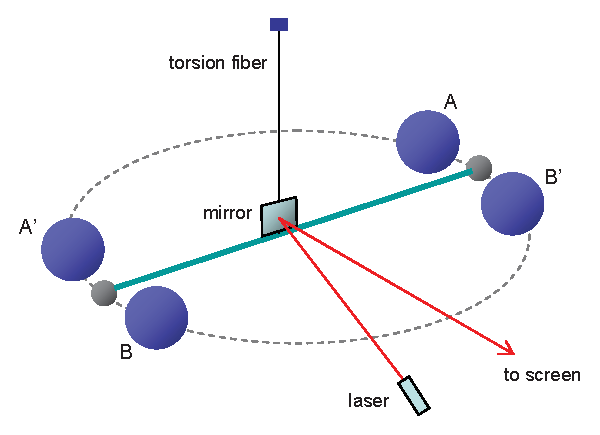
\includegraphics[width=4in]{apparatus3d.eps}
\caption{\label{fig:apparatus3d}
Diagram of the experimental apparatus used to measure the value of G.
The balance beam is free to rotate in the horizontal plane, subject to
the gravitational forces between the fixed and suspended masses, and the
restoring torque from the fiber. 
}
\end{figure}

\begin{figure}
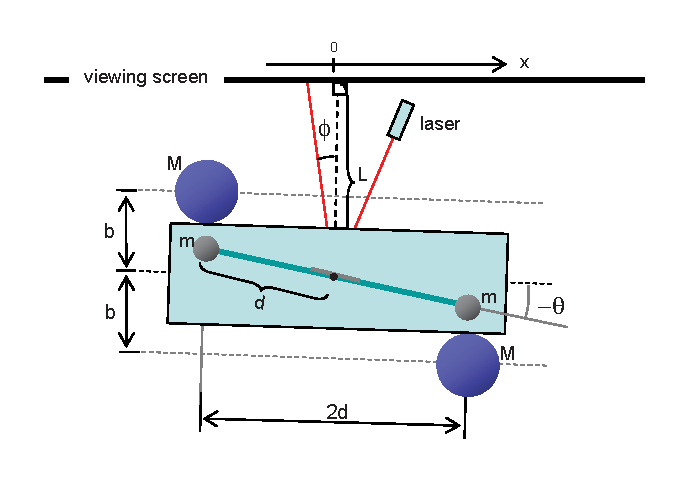
\includegraphics[width=4in]{apparatus2d.eps}
\caption{\label{fig:apparatus2d}
Diagram of the experimental apparatus, viewed from above with the large
masses in positions $A$, and $B$.  The suspension fiber is indicated by
the dot in the center of the figure.  The shaded region is the interior
of the enclosed volume containing the balance beam.  The symmetry axis of
the apparatus is deliberately shown be somewhat misaligned from the plane
of the viewing screen, as is normal for proper alignment.  Some angles are
exaggerated for emphasis.  Distances are not drawn to scale.
}
\end{figure}

\section{Experimental Method}

A diagram of the experimental apparatus is shown in 
Fig.~\ref{fig:apparatus3d}.  Two small lead spheres are attached to
the ends of a light rod which serves as a balance beam.
This rigid dumbbell is suspended horizontally by a vertical
torsion fiber, all enclosed behind transparent walls to protect
the balance from air currents.
The two large lead spheres outside the enclosure gravitationally
attract the inner spheres. Equilibrium is established when the
torque on the dumbbell due to the gravitational forces is
balanced by the restoring torque from the torsion fiber. The
two large spheres can then be rotated from their initial
positions, labeled $A$ and $B$, to the symmetrically located
positions at $A'$ and $B'$. This displaces the equilibrium and the
torsion balance begins to oscillate about a vertical axis.
Attached to the center of the rod is a small mirror. By
observing the deflection of a beam of light reflected from this
mirror, the angular movement of the torsion balance can be
measured.

Fig.~\ref{fig:apparatus2d} shows the distances and angles that must
be measured in the experiment.  The angle $\theta$ of the balance beam
is measured relative to the symmetry axis of the apparatus, as shown.
Place a vertical mark on the viewing screen from which a line perpendicular
to the screen passes through the wire of the balance.  This defines the
origin of the $x$ measurements to be carried out later.  Find the bubble
level, a small round clear plastic disk filled with liquid with a small
bubble of air that appears in the center of the top window when it is level.
Place the bubble level on the top of the rectangular enclosure of the
balance and observe the displacement of the bubble from the center of
the inner circle.  The top surface of the box is not perfectly smooth,
so you should make observations at several positions and take the average.
Level the balance by adjusting the screws in its feet until the bubble in
the level is approximately centered.  Look through the side window of the
box to make sure that the pin marking the mid-point of the balance hangs
freely above the center point.  If you ever need to move the balance while
you are aligning it, move it very slowly and try to minimize vibrations.

Place the laser on a stable support at the same height as the window of
the apparatus and align it so that the beam spot is centered on the mirror
that sits on the balance beam.  The laser should be stable, and once
measurements have begun, it should not be disturbed for the duration
of the experiment.  Make sure that the reflected spot on the viewing
screen is bright and symmetrical.

Make sure that the large lead masses are removed from the holding rings.
Observe the motion of the balance by watching the reflected laser spot
move on the screen.  The natural oscillation period of the balance is
about 10 minutes, so motion of the spot may seem at first to be very slow.
To see if it is moving, hold a finger at the spot position on the viewing
screen; if the spot moves off the finger within 10-15 seconds then the
beam is moving at a reasonable speed.  If somehow it gets moving too fast
or exhibits rapid vibrations, leave the apparatus untouched for 15-20 minutes
and it will settle down on its own.  Watch the motion of the spot for 10
minutes to see one complete period.  The goal in observing these initial
oscillations is to find the limits of motion of the balance beam, and mark
them with vertical lines on the viewing screen.  These outer limits are
caused by the balance beam striking the inside surface of the glass windows
of the enclosure.  You know when this happens because the beam spot on the
viewing screen appears to ``bounce'', suddenly reversing its direction at
a certain point.

If the balance has been sitting quietly for more than an
hour, the oscillations may have decayed away to the point that it never 
reaches the window on one side or the other, or both.  If you
suspect that this is the case, gently tap the glass sides of the balance
enclosure.  After the vibrations settle down, you should see that the slow
oscillation amplitude has increased.  Repeat this until you clearly see the
spot bouncing from both ends of its oscillation range.  If it gets moving too
fast, the end-point positions will appear to be different on each swing, but
once it settles down, the end-points will be reproducible to better than the
size of the laser spot.  Mark the limits with vertical lines on the screen.
Make sure that the oscillation range between the two limits is reasonably
close to centered on the $x=0$ mark you made earlier, within 2-3\%.  If
this is not the case, move the laser (not the balance) until the full range
of the spot motion is centered on $x=0$ at the 2-3\% level.  If you moved
the laser, redraw the new limits on the viewing screen.  The $x=0$ mark
should not be moved.

At this point, the alignment of the apparatus is nearly complete.  Note
that the central plane of the apparatus is not exactly parallel to the
viewing screen.  These two planes are normally misaligned by a small angle,
as suggested by the slight tilt from horizontal of the dashed lines in 
Fig.~\ref{fig:apparatus2d}.  This is properly taken into account in the data
analysis.

Set up the camera that will be used to measure the motion of the beam spot
using time-lapse photography.  Set the time-lapse interval to 5 seconds.
Place a meter stick next to the viewing screen within the view window of
the camera, to be used to set the scale later when analyzing the images.
Set the zoom on the camera so that both limits of the laser spot motion
marked earlier are just within the viewport.  Disable the flash and set
the resolution to $640\times 480$ pixels.  Begin a measurement sequence
with the camera, with no exterior weights loaded on the balance.  Watch
the first couple of oscillations of the laser spot.  Review the sequence
of images taken with the camera, and visually estimate where the mid-point
of the oscillations is located on the screen.  This needs to be close to the
$x=0$ point on the screen, within $\pm$10\% of the distance between the
limit points.

If the apparatus has not been aligned for several days, this
usually requires adjustment of the zero-point of the torsion wire.  This is
adjusted by turning the large knurled nut at the top of the central tube on
the balance.  Without shaking the balance, carefully loosen the plastic lock
nut, then turn the knurled nut in the direction you want the zero-point to
shift.  Usually one over-estimates how much rotation is needed, so start off
with a very small adjustment, and increase it as needed.  After each 
adjustment, tighten the lock nut again to hold the zero-point fixed.  Finding
the zero point and getting it properly centered on the screen is the most
time-consuming aspect of this entire experiment.  Exercising patience at
this stage and getting the alignment right will pay off later.  Once the
zero-point has been found and centered, the alignment is complete and should
not be touched.  At some later point during the experiment you may notice that
the zero-point seems to have shifted somewhat.  This is caused by long-term
``memory'' in the torsion fiber, and can be taken into account in the data
analysis.  If you ever redo the alignment, you must start the data-taking
again from the beginning.

Check the image sequence recorded by the camera to make sure that the zoom,
focus, brightness, and snapshot interval settings are optimal, then start
a measurement run.  A recording run consists of a continuous sequence of 
images taken without moving the camera, the laser, or the balance.  To be
useful, a measurement run should subtend at least 5 complete oscillations,
requiring no less than 1 hour of continuous observation with the camera,
and 500-1000 images.

Software tools for converting the still images to a speed-up video of the
run are provided on the laboratory computers.  Create and view the video
of the initial run taken without weights present.  A slight drift in the
zero-position of the oscillations is inevitable and will be taken into account
in the data analysis.  If the drift is so large that there is a risk that
the beam will run into the limit points before the oscillations die away,
the apparatus will need to be allowed to settle for a day or two, after which
you should repeat the zero-point alignment, and start the measurements again.
Once you are satisfied with the results from the initial run, save the
movie for later analysis under the name {\tt unloaded\_1}.  The software
script that generates the movie from the time-lapse sequence also reports the
average interval between frames.  Be sure to record this number in your
log book for each run, so that you can convert later from frame number to
seconds.

Use a tape measure to record the distance $L$ from the torsion fiber to the
viewing screen, together with its uncertainty.  Measure the masses $M$ of
the two external lead spheres.  You should find that the two masses are equal
within the uncertainty $\Delta M$ of your measurement.  Record $M$ and
$\Delta M$.  Measure the distance $2d$ by holding a ruler up to the glass
window of the balance and sighting the centers of the two spheres along the
rules on the ruler.  Have more than one experimenter repeat the measurement,
and share the results only after all measurements have been made, recording
the average value as the value of $2d$ and the RMS of your measurements 
divided by $\sqrt{N}$ as its uncertainty.

The most difficult distance to measure in this experiment --
and the most critical in terms of its effect on the uncertainty of the 
final result -- is the determination of the distance $b$.  To measure this,
place the two lead spheres in their holder on the balance, and swivel the
holder until the lead spheres barely touch the glass on both sides.  Over
years of use, these lead spheres have many bumps and bruises on their surface
so their radii are not uniform.  You may need to turn them several times
until you find smooth spots where both spheres come into contact with the
glass at the same time.  Check that this is the case in both the front-left
and front-right orientations.  Once they have been placed, do not move the
external spheres in the holder again until after the gravitational
measurements are complete.  Once they are placed, swivel the holder out away
from the glass and use a vernier caliper to measure the diameter of the two
spheres along the axis containing the points where they touch the glass.
Record average of the two measurements together with its
uncertainty.  Use the vernier caliper to measure the total thickness of the
housing, including the glass windows, and record this together with its
uncertainty.  Compute the sum of the housing thickness plus the sphere
diameter and record this value as $2b$, together with its uncertainty.

Move the external mass holder to the front-left position, with the mass
just barely touching the glass, and start a new run with the camera.  When
this run is complete, without stopping the camera, rotate the mass holder
to the front-right position and take a second run.  Save the images, and
convert them to video format, recording the average interval between frames
as reported by the video conversion script.  Remove the two external masses
and set them aside on a bench, then take a new run with the camera, called
{\tt unloaded\_2}.  When these images are converted to video format and
the frame interval recorded, you are finished with the data collection
phase of the experiment.

\section{Theoretical Model}

Consider the apparatus represented in Fig.~\ref{fig:apparatus2d}.  The 
positions of the small spheres mounted on the ends of the balance beam
are denoted as $\vec{x}_1$ and $\vec{x}_2$, where $\vec{x}_1$ refers to 
the mass on the right in the figure.  The positions of the large spheres
are denoted as $\vec{y}_1$ and $\vec{y}_2$, where $\vec{y}_1$ refers to
the sphere on the lower side of the enclosure in the figure.  All of these
vectors lie in the same plane, taken to be $z=0$.  The origin
of the coordinate system is the intersection of the torsion wire axis
with the $z=0$ plane.  In the orientation shown in the figure,
\begin{eqnarray}
\vec{x}_1 &=& (d\cos\theta,d\sin\theta)
\nonumber \\
\vec{x}_2 &=& (-d\cos\theta,-d\sin\theta)
\nonumber \\
\vec{y}_1 &=& (d,-b)
\nonumber \\
\vec{y}_2 &=& (-d,b)
\end{eqnarray}
According to Newton's universal law of gravitation, the presence of the
external spheres produces a net force on the balance mass at $x_1$ that
is given by
\begin{equation}
\vec{F}_1 = GMm\left[
\left(\frac{\vec{y}_1-\vec{x}_1}{|\vec{y}_1-\vec{x}_1|^3}\right)+
\left(\frac{\vec{y}_2-\vec{x}_1}{|\vec{y}_2-\vec{x}_1|^3}\right)
\right]
\label{eq:F1}
\end{equation}
where $M$ is the mass of the large spheres and $m$ is the mass of the small
spheres on the ends of the balance beam.  The gravitational force on the rod
connecting the two small spheres is neglected in this analysis.
A similar expression gives the force $\vec{F}_2$ that the two external masses
produce on the small mass on the other end of the balance beam at $\vec{x}_2$,
obtained from Eq.~\ref{eq:F1} by replacing $\vec{x}_1$ everywhere with
$\vec{x}_2$.  The fact that $\vec{x}_1=-\vec{x}_2$ and $\vec{y}_1=-\vec{y}_2$
implies that $\vec{F}_1=-\vec{F}_2$, so the net force on the balance beam is
zero.  The net torque, however, does not sum to zero.  Consider just the
torque on the balance beam about the origin that arises from force $\vec{F}_1$.
\begin{eqnarray}
\vec{\tau}_1 &=& GMm\left[
\vec{x}_1\times
\left(\frac{\vec{y}_1-\vec{x}_1}{|\vec{y}_1-\vec{x}_1|^3}\right)+
\vec{x}_1\times
\left(\frac{\vec{y}_2-\vec{x}_1}{|\vec{y}_2-\vec{x}_1|^3}\right)
\right]
\nonumber\\
&=& GMmDd\left[
\frac{-\sin(\theta+\theta_M)}{|\vec{y}_1-\vec{x}_1|^3}+
\frac{\sin(\theta+\theta_M)}{|\vec{y}_2-\vec{x}_1|^3}
\right]\hat{z}
\end{eqnarray}
where $D^2=d^2+b^2$ and $\theta_M=\sin^{-1}(b/D)$.
The torque $\vec{\tau}_2$ on small mass 2 is the same, leading to the
following expression for the net gravitational torque on the balance
beam.
\begin{equation}
\vec{\tau}_G = -2GMmDd\;\sin(\theta-\theta_M)\left[
\frac{1}{|\vec{y}_1-\vec{x}_1|^3}-
\frac{1}{|\vec{y}_2-\vec{x}_1|^3}-
\right]\hat{z}
\end{equation}
In this analysis, gravitational forces from all of the other objects
surrounding the apparatus, including the camera, the support for the
apparatus, the building in which the experiment is housed, and
significant geological features in the local region, the moon, the earth
itself, the sun, etc., all of which may be expected to produce gravitational
forces at least as large as those from the lead sphere, or even larger.
To understand why these background forces do not affect the experiment,
note that the alignment procedure guarantees that the net gravitational
force from all of the neglected external objects has a zero projection
onto the rotation plane of the balance.  This is because a freely hanging
wire naturally aligns with the direction of the net force, and the balance
is constrained to move such that the height of its center of mass remains
fixed.

This leaves open the question of the net background torque.  This torque
does not sum to zero, and may be larger than the torque from the lead
spheres, but it does not matter because it is canceled exactly by an
opposite torque $\vec{\tau}_w$.  The torsion wire produces a harmonic
restoring torque that attracts the beam back toward its equilibrium
orientation $\theta_0$.
\begin{equation}
\vec{\tau}_w = -K(\theta-\theta_0)
\label{eq:hooke}
\end{equation}
The presence of a constant external torque simply shifts the equilibrium
position $\theta_0$ such that it is completely canceled out by the wire.
From this point of view, it is impossible to measure the $\theta_0$ of the
wire itself because it is impossible to get rid of all of the background
gravitational torques.  Thus, when we measure the point $\theta_0$ in the
presence of this background but without the lead spheres present, we are
effectively measuring the net background torque and getting rid of its 
effect on the experiment.  This justifies ignoring all other masses except
the ones that are moved during the experiment.  Keep in mind that other
things in the environment that move during the experiment, including human
bodies, can throw off the results.  Thus it is suggested that everyone keep
away from the vicinity of the balance during periods of measurement with
the camera.

When both the gravitational torque $\vec{\tau}_G$ and $\vec{\tau}_w$ are
taken into account, the condition for static equilibrium of the balance
becomes
\begin{equation}
K(\theta-\theta_0)=-2GMmDd\;\sin(\theta+\theta_M)
\left(\frac{1}{r_1^3}-\frac{1}{r_2^3}\right)
\label{eq:equil0}
\end{equation}
where
\begin{eqnarray}
r_1^2 &=& d^2(1-\cos\theta)^2 + (b+d\sin\theta)^2
\nonumber\\
r_2^2 &=& d^2(1+\cos\theta)^2 + (b-d\sin\theta)^2
\label{eq:r12}
\end{eqnarray}
A system obeying Eq.~\ref{eq:hooke} in the form of Hooke's Law undergoes
simple harmonic motion with a natural frequency given by
\begin{equation}
\omega=\sqrt{\frac{K}{I}}
\end{equation}
where the moment of inertia $I$ of the beam can be very well approximated
as $2md^2$.  The angular frequency $\omega$ of the beam oscillations is
easier to measure than $K$, so the equilibrium condition Eq.~\ref{eq:equil0}
can be rewritten as
\begin{equation}
\theta-\theta_0=-\frac{GMD}{d\omega^2}\sin(\theta+\theta_M)
\left(\frac{1}{r_1^3}-\frac{1}{r_2^3}\right)
\label{eq:equil1}
\end{equation}
It turns out that in the experiment one does not measure $\theta$ directly.
Instead one measures the position of a laser spot on a viewing screen, which
can easily be converted into the angle $\phi$ shown in
Fig.~\ref{fig:apparatus2d}.
\begin{equation}
\phi=\phi_c+2\theta
\end{equation}
where the constant offset $\phi_c$ incorporates a number of unmeasured
offsets, including the angle between the mirror and the balance beam axis,
the angle between the mid-plane of the balance enclosure and the viewing
plane, and the incidence angle of the laser in the frame of the apparatus.
While all of these offsets are not individually measured in the experiment,
their sum $\phi_c$ is measured as the angle $\phi$ corresponding to the
midpoint between the two limits in $\phi$ where the ends of the beam strike
the glass walls of the enclosure.

Measuring the average value $\phi_0$ about which the beam oscillates when the
external masses are removed allows the value of $\theta_0$ to be 
determined as
\begin{equation}
\theta_0=\frac{1}{2}(\phi_0-\phi_c)
\end{equation}
Placing the external masses in their supports and rotating them to the
front-left position leads to the beam oscillating with the same period about
a new equilibrium $\theta_1$, corresponding to observed angle $\phi_1$ of
the spot on the viewing screen.
\begin{eqnarray}
\theta_1 &=& \frac{1}{2}(\phi_1-\phi_c)
\nonumber\\
&=& -\frac{GMD}{d\omega^2}\sin(\theta_1+\theta_M)
\left(\frac{1}{r_1^3}-\frac{1}{r_2^3}\right)
\label{eq:theta1}
\end{eqnarray}
Similar relations hold for the front-right configuration of the external
masses, for which the shifted equilibrium position is labeled $\theta_2$.
\begin{eqnarray}
\theta_2 &=& \frac{1}{2}(\phi_2-\phi_c)
\nonumber\\
&=& -\frac{GMD}{d\omega^2}\sin(\theta_2-\theta_M)
\left(\frac{1}{s_1^3}-\frac{1}{s_2^3}\right)
\label{eq:theta2}
\end{eqnarray}
where the distances $s_1$,$s_2$ are defined in a similar manner to the
$r_1$,$r_2$ in Eq.~\ref{eq:r12} as
\begin{eqnarray}
s_1^2 &=& d^2(1-\cos\theta)^2 + (b-d\sin\theta)^2
\nonumber\\
s_2^2 &=& d^2(1+\cos\theta)^2 + (b+d\sin\theta)^2
\end{eqnarray}
Note that $r_1$ and $r_2$ must be evaluated at angle $\theta=\theta_1$ in 
Eq.~\ref{eq:theta1}, whereas $s_1$ and $s_2$ in Eq.~\ref{eq:theta2}
must be evaluated at $\theta=\theta_2$.  
Solving Eqs.~\ref{eq:theta1} and \ref{eq:theta2} for $G$
yields two independently measured values for this important physical constant.

\section{Data Analysis}

Use the Open Source Physics Tracker~\cite{tracker} application to analyze
the three image sequences, {\tt unloaded\_1, left\_right, and unloaded\_2},
and digitize the position of the laser spot as a function of frame number.
Be sure to set the scale and orientation of the axes in the image, using
the meter stick that is visible in the image, before starting the
autotracker.  Save the results from each run into output files containing
3 columns of data for $t$, $x$ and $y$.  Import these data into three
separate worksheets in a spreadsheet application for further analysis.
Correct the $t$ columns on each sheet to reflect the correct time interval
between frames for that run.  The $y$ columns can be eliminated.

On the {\tt unloaded\_1} worksheet, create a new column for the angle
$\phi$ and fill in its values using the formula,
\begin{equation}
\phi=-\tan^{-1}\left(\frac{x}{L}\right)
\label{eq:phidef}
\end{equation}
where $L$ is the perpendicular distance from the torsion fiber to the
screen.  Locate the midpoint $x_c$ between the two limits marked on the
viewing screen, and record the value of $\phi_c$ obtained from it using
Eq.~\ref{eq:phidef}.  Be sure to record the measurement errors on each.

Plot the sequence $\phi$ {\em vs} $t$ and verify that the
equilibrium position around which the oscillations are centered is
reasonably stable throughout the run.  Carry out a least-squares fit
of these $\phi$ data to the following model function,
\begin{equation}
\Phi(t) = a_0 e^{-\lambda_0 t}\sin(\omega(t-t_0)) + a_1 e^(-\lambda_1 t)
+a_{\infty}
\label{eq:fitfunc}
\end{equation}
where free parameters $a_0$, $\lambda_0$, $\omega$, $t_0$, $a_1$, $\lambda_1$,
and $a_{\infty}$ are varied to minimize the $\chi^2$.  To define the $\chi^2$,
you need to estimate the measurement error on $\phi$.  This should be
determined mainly by the error on the $x$ position of the laser spot,
propagated through Eq.~\ref{eq:phidef}.  A fraction of the laser spot
diameter would be a good starting point for this estimate.  A good way
to check your estimate is to compare the minimum $\chi^2$ value returned
from the fit with the number of degrees of freedom $N$ in the fit.  These
two should not match exactly, but the agreement should be within roughly
$\pm\sqrt{2N}$.  Plot the best-fit curve on top of the data and verify visually 
that the fit was successful.  Deviations between the data points and the
fit curve should scarcely be visible in the plot.

If deviations are apparent, try excluding a sequence of points from the
fit starting at the beginning of the run.  It may be that the balance was
still shaking from the initial setup, and needed time to settle down.
To exclude a range of data from the fit, simply redefine the $\chi^2$ cell
in the spreadsheet to exclude those rows from the sum. Do not remove these
points from the graph, as it is interesting to see what happens to the
agreement between the curve and the data in regions where the data are
excluded from the fit.  In the end, your fit should cover at least the
last 3 complete oscillations of the system.  It is not legitimate to
``cut out'' data from the middle of the run, just because they do not
agree with the model.  The only part you may exclude is an initial sequence,
and only because it may be affected by transients.

Carry out a jack-knife analysis to obtain the errors on each of the fit
parameters.  In a case like this, with hundreds of points in the data set,
it is sufficient to carry out only 5-10 jack-knife fits.  To do 10 fits,
free up a block on your spreadsheet with 12 columns and 10 rows.  Label the
first column $\chi_s^2$ and assign it the formula equal to the overall
$chi_s^2$ cell minus the sum of {\em every tenth entry in the residuals
squared column}.  Entering a formula to do this requires a little
spreadsheet magic using the {\tt SUMPRODUCT} and {\tt MOD}
built-in functions.  You should be able to figure this out, or find a
recipe for how to do it online.  Copy this formula down all 10 rows of
the block, then carry out 10 fits to minimize the 10 $\chi_s^2$ functions
so defined.  After each fit, copy the best-fit values of the 11 free
parameters into the 11 columns to the right of the $\chi_s^2$ column.
When you are done, the error on the 11 free fit parameters can be
computed, based on the standard deviation of the corresponding column
in the jack-knife fit results block, in the usual fashion for jack-knife
error analysis.

Repeat the above analysis for the data from the {\tt unloaded\_2} run.
Check whether the oscillation frequency $f$ and the two damping constants
$\lambda_0$ and $\lambda_1$ are consistent between the two unloaded runs.
If this is not the case, investigate the source of the inconsistency, and
find a way to include it in the errors that you assigned to the measured
coordinates.  Once these two independent fits are seen to be consistent
with one another, you are ready to do a joint fit to the front-left and
front-right data sets.

Import the {\tt left,right} data for $t,x,y$ into a fresh worksheet.  
Prepare the data for fitting in the same fashion as before, correcting $t$
to represent real time, eliminating $y$, and converting $x$ and $\Delta x$
into $\phi$ and $\Delta\phi$.  Graph the measured values of $\phi$ {\em vs}
$t$ on a single plot, showing the oscillations around the left equilibrium
point, followed by the right.  Set up two identical side-by-side
parameter blocks representing the free parameters in Eq.~\ref{eq:fitfunc}.
The first set will be used to fit the first half of the data in this worksheet,
and the second set to fit the second half.  As before, form a single column
for the fit function $\Phi(t)$ and enter the formula from Eq.~\ref{eq:fitfunc}.
Half-way down the column, near where the weights were switched from left to
right, edit the fit formula to use the second parameter set instead of the
first, then copy this formula down the rest of the column.  Enter beginning
guesses for the values in the parameter blocks, then plot the approximate
fit function on top of the measured points in the graph.

In the cell for the $\chi^2$ value for parameter block 1, enter the sum of
the residual squares for the first half of the data.  You should only include
in this sum the rows that correspond to the region of clean behavior,
excluding points early in the run period that might have been contaminated
by transients, and also points when you intervened to switch between the two
mass configurations.  You should only exclude data from the beginning of the
run and during the transition period between the two configurations; do not
clip data out of the middle of one of the oscillation periods.

Carry out independent fits of the two oscillation periods within run 2,
using parameters from the two parameter blocks.  Refine the ranges included
in the $\chi^2$ sums until the fits show no major systematic deviations
from the data.  Then verify that the measurement error you used on the
$x$ values makes sense by comparing the best-fit $\chi^2$ value with
the number of degrees of freedom.  Repeat the jack-knife error analysis
for both of these periods.

In the next step, you will introduce the constraint that the values of
the frequency and damping rates should be the same before and after the
lead masses where switched.  Henceforth subscript 1 will be used to denote
parameters in the first block, and 2 to label those in the second block.
In the place of the guessed value you entered for $\omega[2]$ in the second
parameter block, create a formula equating it to $\omega[1]$ in the first
block.  Do the same thing for $\lambda_0[2]$ and $\lambda_1[2]$, constraining
them to always equal $\lambda_0[1]$ and $\lambda_1[1]$, respectively.  In a
new cell, form a global $\chi_T^2$ as the sum of the original $\chi^2[1]$
and $\chi^2[2]$ values, and do a least-squares fit on the value of $\chi_T^2$,
allowing only the 11 unconstrained parameters to vary, 7 from parameter block
1 and 4 from block 2.

Use the jack-knife technique to estimate the errors on the 11 parameters
returned from the global fit.  You should find that introducing the
constraints between the two parameter blocks and fitting both sets at once
results in somewhat smaller errors on the fit parameters than were obtained
fitting the two periods separately.  The parameters of particular interest
in extracting a value for $G$ are the frequency $\omega$ and the two
offset values $a_{\infty}[1]$ and $a_{\infty}[2]$.

Use a similar jack-knife analysis on the {\tt unloaded\_1} and
{\tt unloaded\_2} data sets, and extract errors on the value of $a_{\infty}$
for the unloaded case.  Verify that the values from the early and later
run periods are in agreement within errors.  To help distinguish between the
different values for $a_{\infty}$ coming from the different fits, they will
be renamed as follows.  The average of $a_{\infty}$ from the {\tt unloaded\_1}
and {\tt unloaded\_2} fits will be called $\phi_0$ and its error
$\Delta\phi_0$.  The value of $a_{\infty}[1]$ from the first fit parameter
set from the weighted run (front-left) will be called $\phi_1$, and that from
the second parameter set (front-right) will be called $\phi_2$.
Their associated errors are $\Delta\phi_1$ and $\Delta\phi_2$, respectively.

To obtain $G$, first convert $\phi_0$, $\phi_1$, and $\phi_2$ into $\theta_0$,
$\theta_1$, and $\theta_2$ using Eq.~\ref{eq:phidef}, being careful to
propagate their errors correctly.  Use Eqs.~\ref{eq:theta1} and \ref{eq:theta2}
and the measured values of all other relevant experimental quantities to
to extract the value of $G$ from your measurements.  You should obtain two
independent estimates for $G$, one from $\theta_1$ and the other from
$\theta_2$.  Compute the error on each of these estimated values, and verify
that the two are in agreement within their errors.

\begin{acknowledgments}
This document was written by Prof.\ Richard Jones, based on an earlier
write-up developed by Profs. Ed Eyler and Doug Hamilton.
\end{acknowledgments}

%% Create the reference section using BibTeX:
%\bibliography{revtex4}

\begin{thebibliography}{9}

\bibitem{Adelberger2009}
E.G.~Adelberger, J.H.~Gundlach, B.R.~Heckel, S.~Hoedl, and S.~Schlamminger,
``Torsion Balance Experiments: A Low-energy Frontier of Particle Physics'',
Prog. Part. Nucl. Phys., Vol. 62, Issue 1 (2009) 102-134.

\bibitem{tracker}
D. Brown, in Open Source Physics: A User's Guide with Examples (2006),
WWW Document, 
(\url{http://www.compadre.org/Repository/document/ServeFile.cfm?ID=7379&DocID=530}).

\end{thebibliography}

\end{document}
%%
%% ****** End of file template.aps ******
%
%
